\subsection{Pairs plots}\label{sub_pairsplots}

%   MODEL 2

\begin{figure}[ht]
\centering
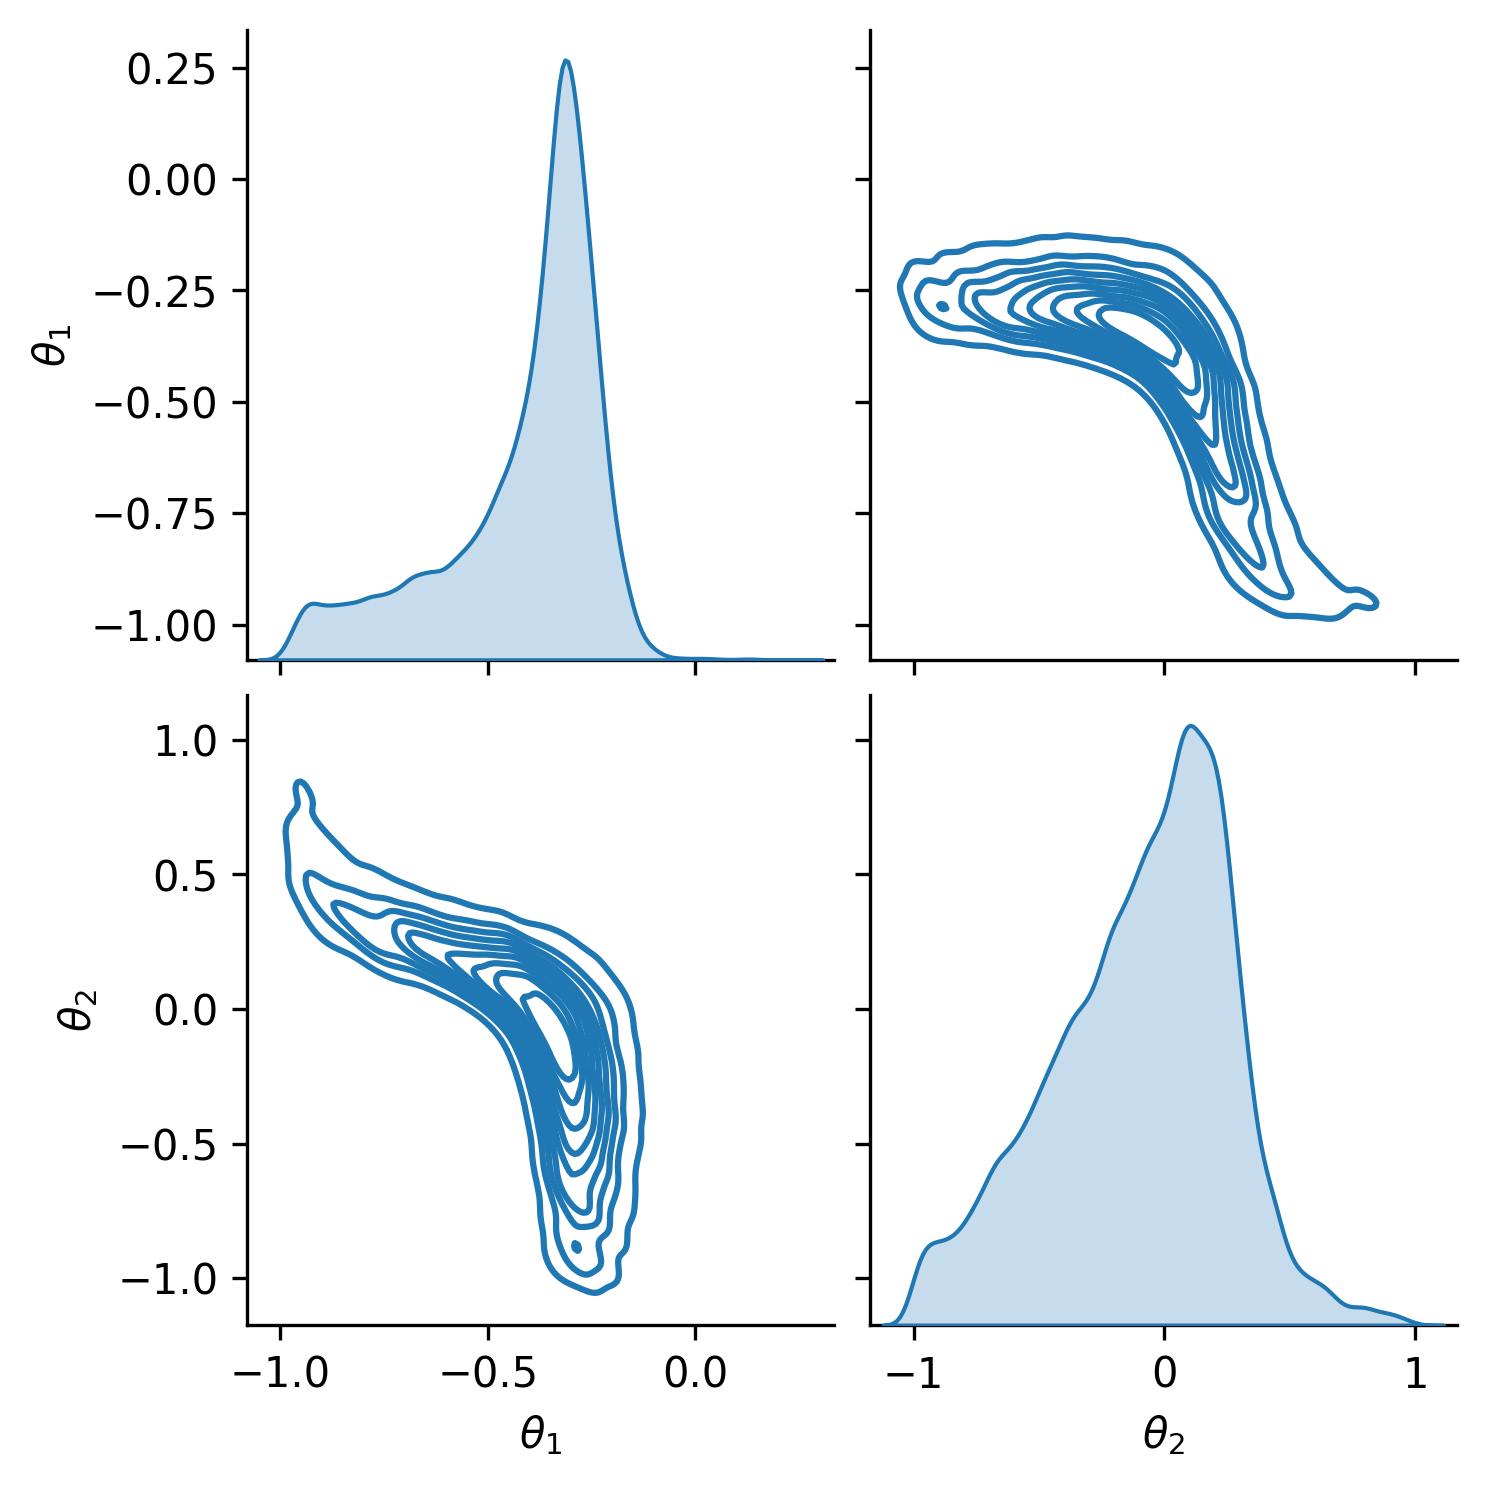
\includegraphics[width=1.0\linewidth]{Figures/appendix_figs/kde_model2_DE.png}
\caption{Pair plots (with a kernel density style) for all calibrated parameters of Model 2. The presented data is from 5 ensembles (last 1000 steps of each chain), run with DE, an uninformative prior and 1 observation for evaluating the likelihood. The parameters as presented here are transformed for MCMC.}\label{fig_kde_model2_DE}
\end{figure}


\begin{figure}[ht]
\centering
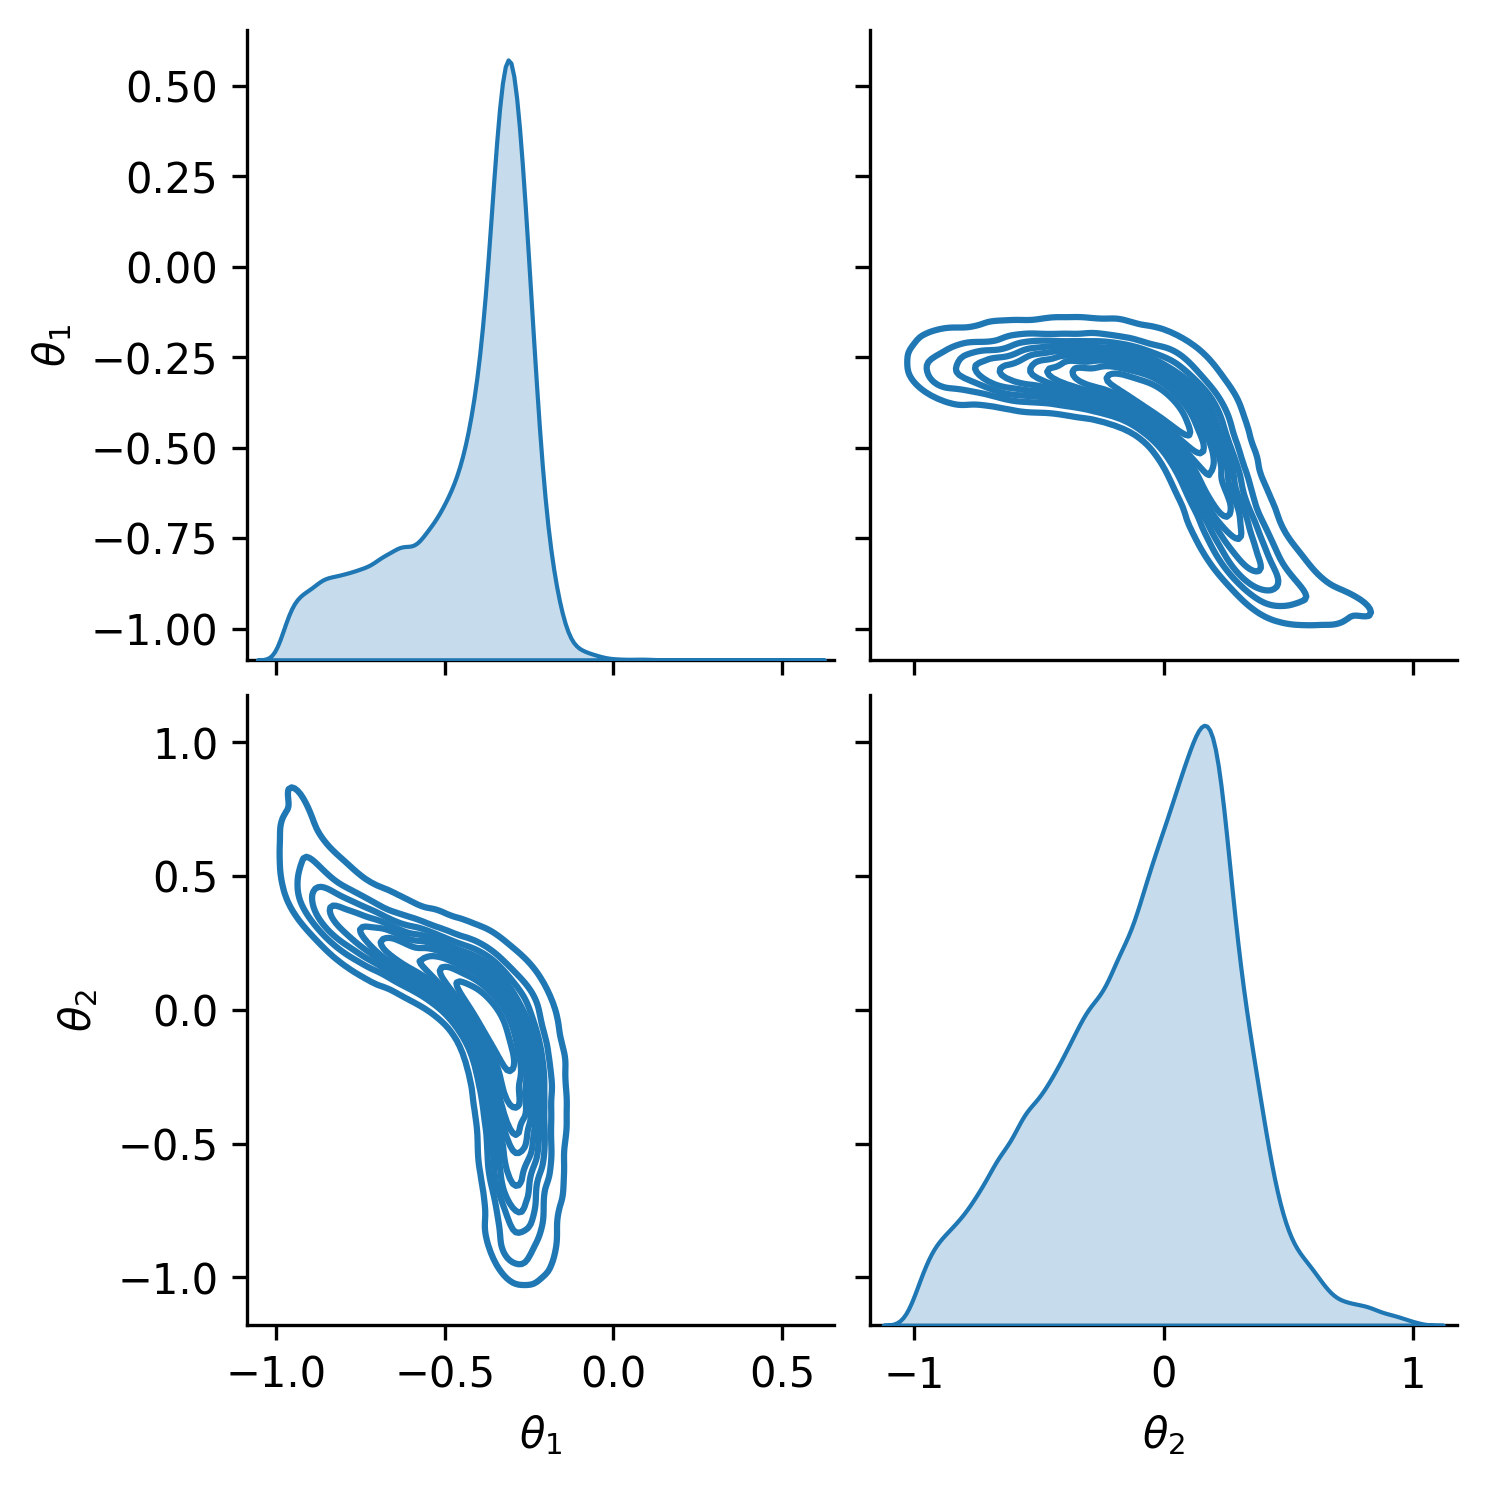
\includegraphics[width=1.0\linewidth]{Figures/appendix_figs/kde_model2_Stretch.png}
\caption{Pairs plots (with a kernel density style) for all calibrated parameters of Model 2. The presented data is from 5 ensembles (last 1000 steps of each chain), run with AI, an uninformative prior and 1 observation for evaluating the likelihood. The parameters as presented here are transformed for MCMC.}\label{fig_kde_model2_AI}
\end{figure}

%   MODEL 3

\begin{figure}[ht]
\centering
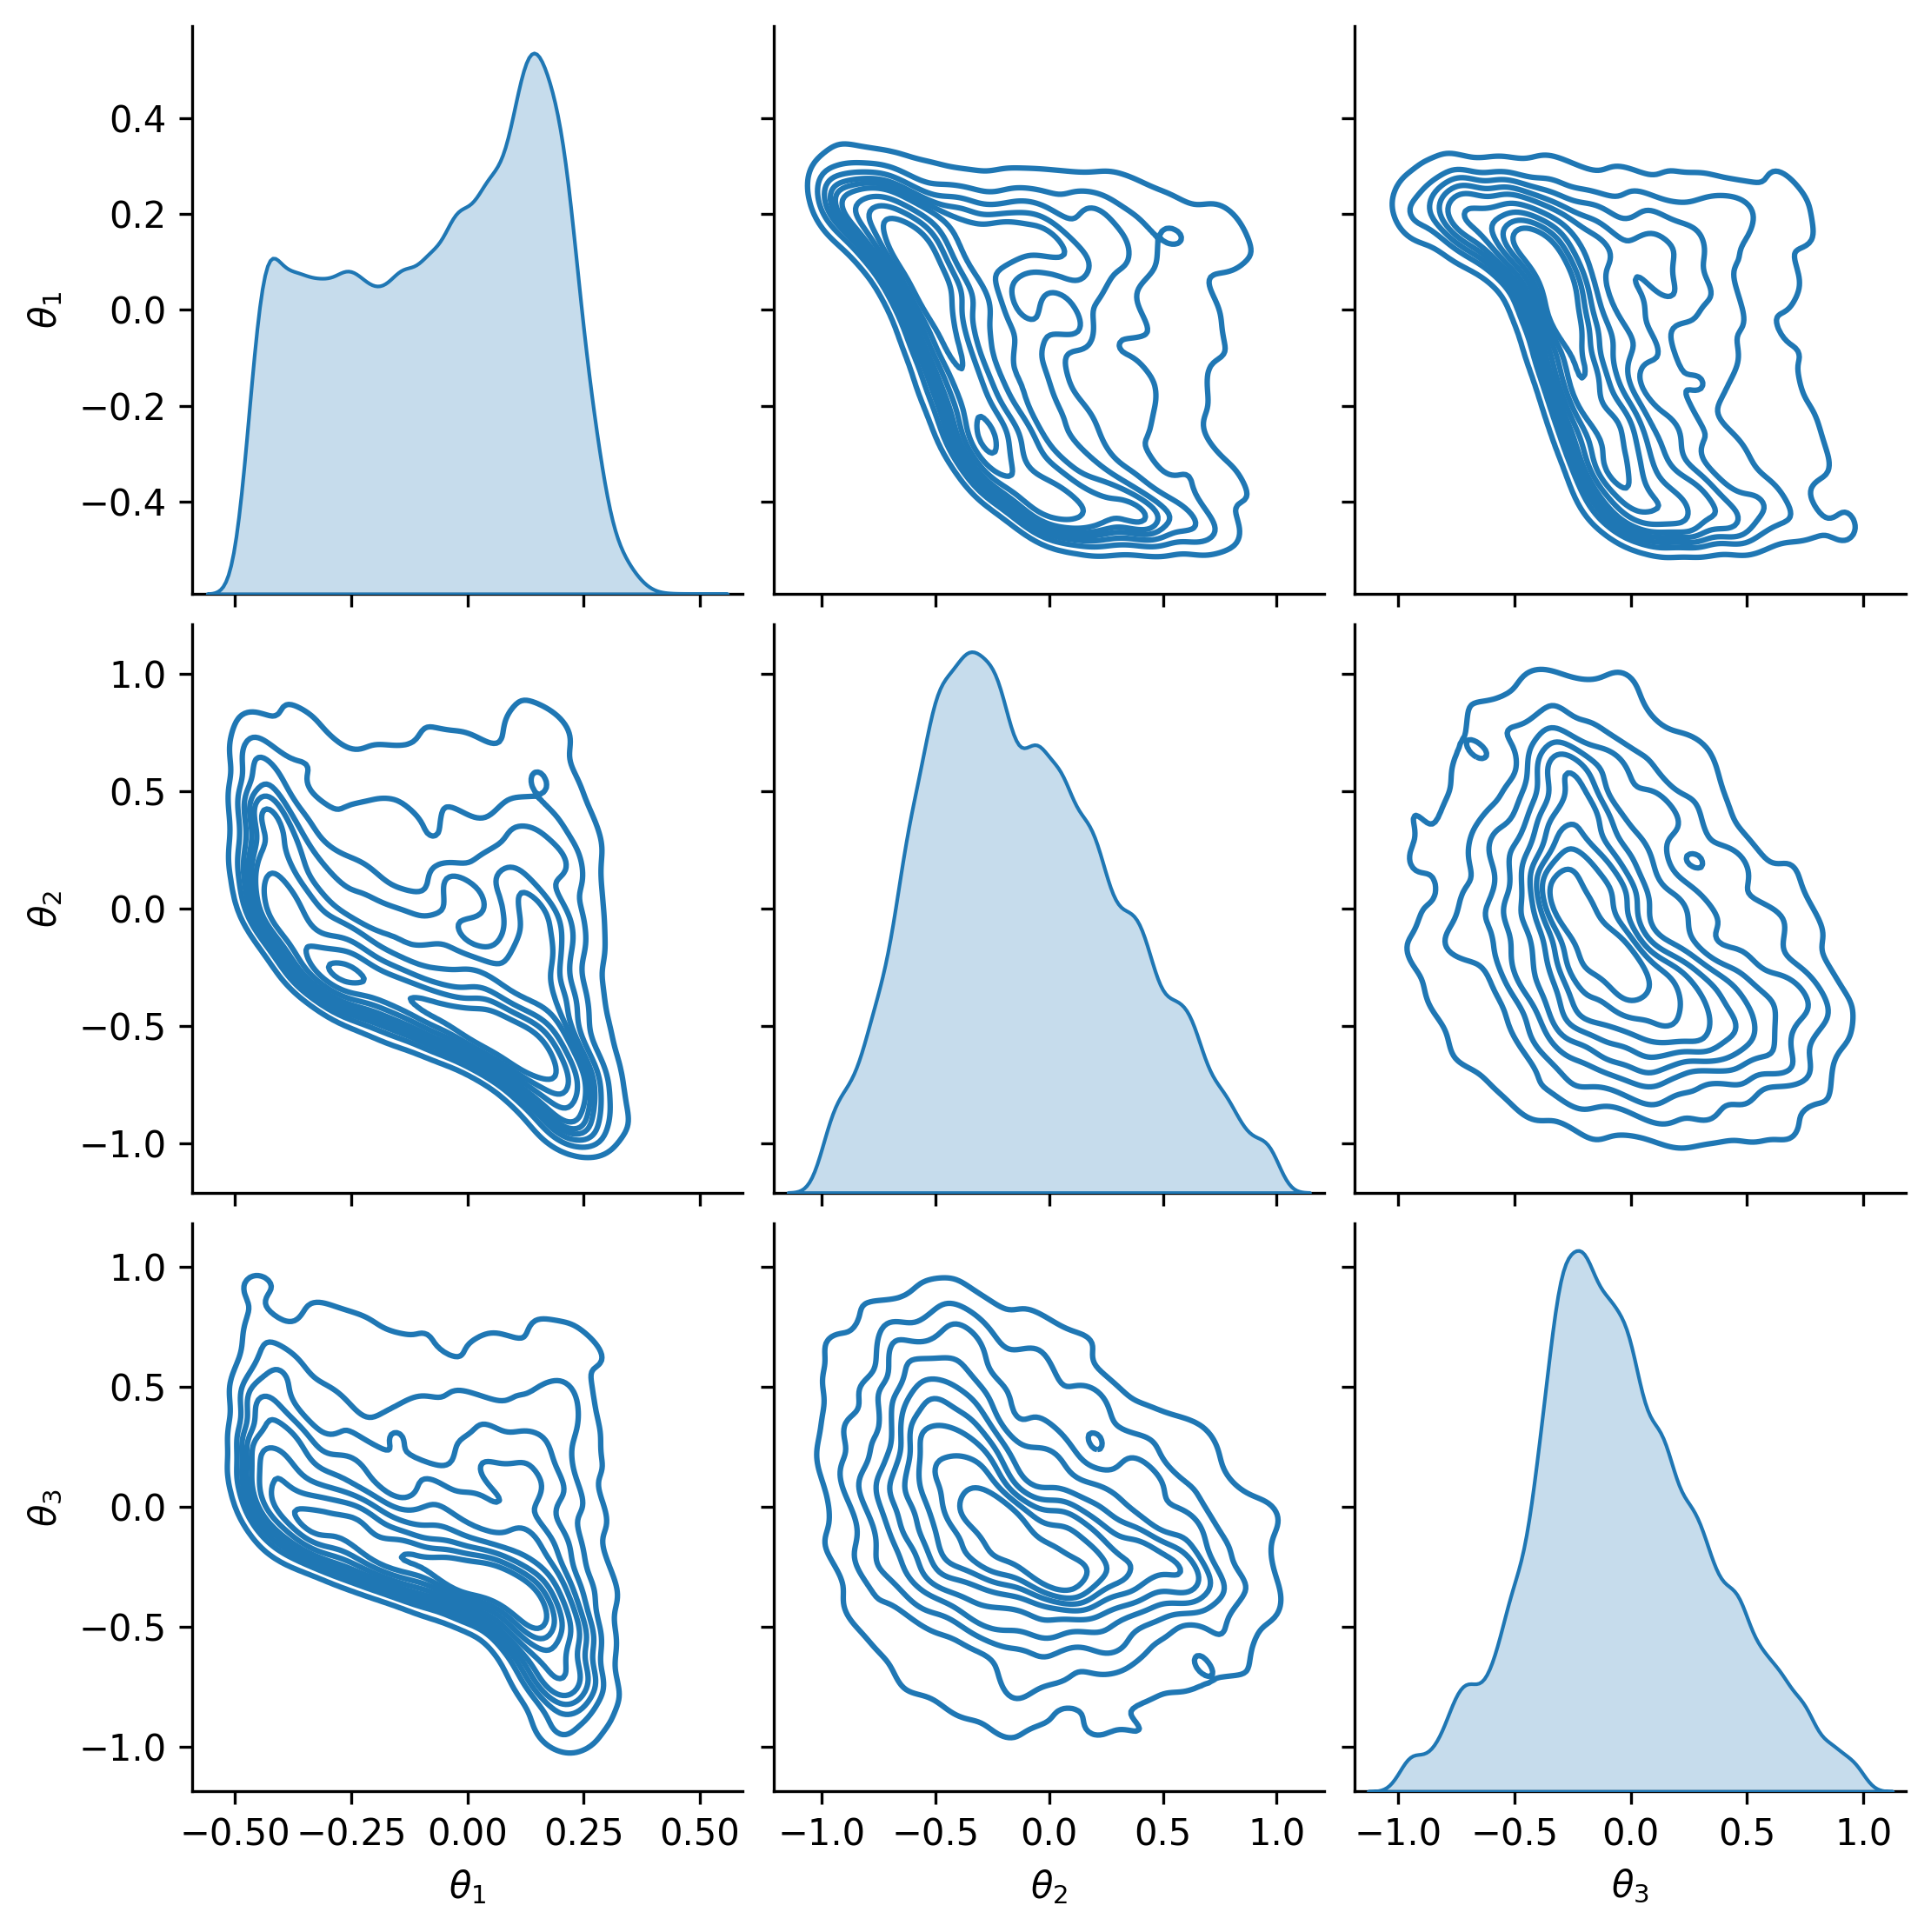
\includegraphics[width=1.0\linewidth]{Figures/appendix_figs/kde_model3_DE.png}
\caption{Pairs plots (with a kernel density style) for all calibrated parameters of Model 3. The presented data is from 5 ensembles (last 1000 steps of each chain), run with DE, an uninformative prior and 1 observation for evaluating the likelihood. The parameters as presented here are transformed for MCMC.}\label{fig_kde_model3_DE}
\end{figure}

\begin{figure}[ht]
\centering
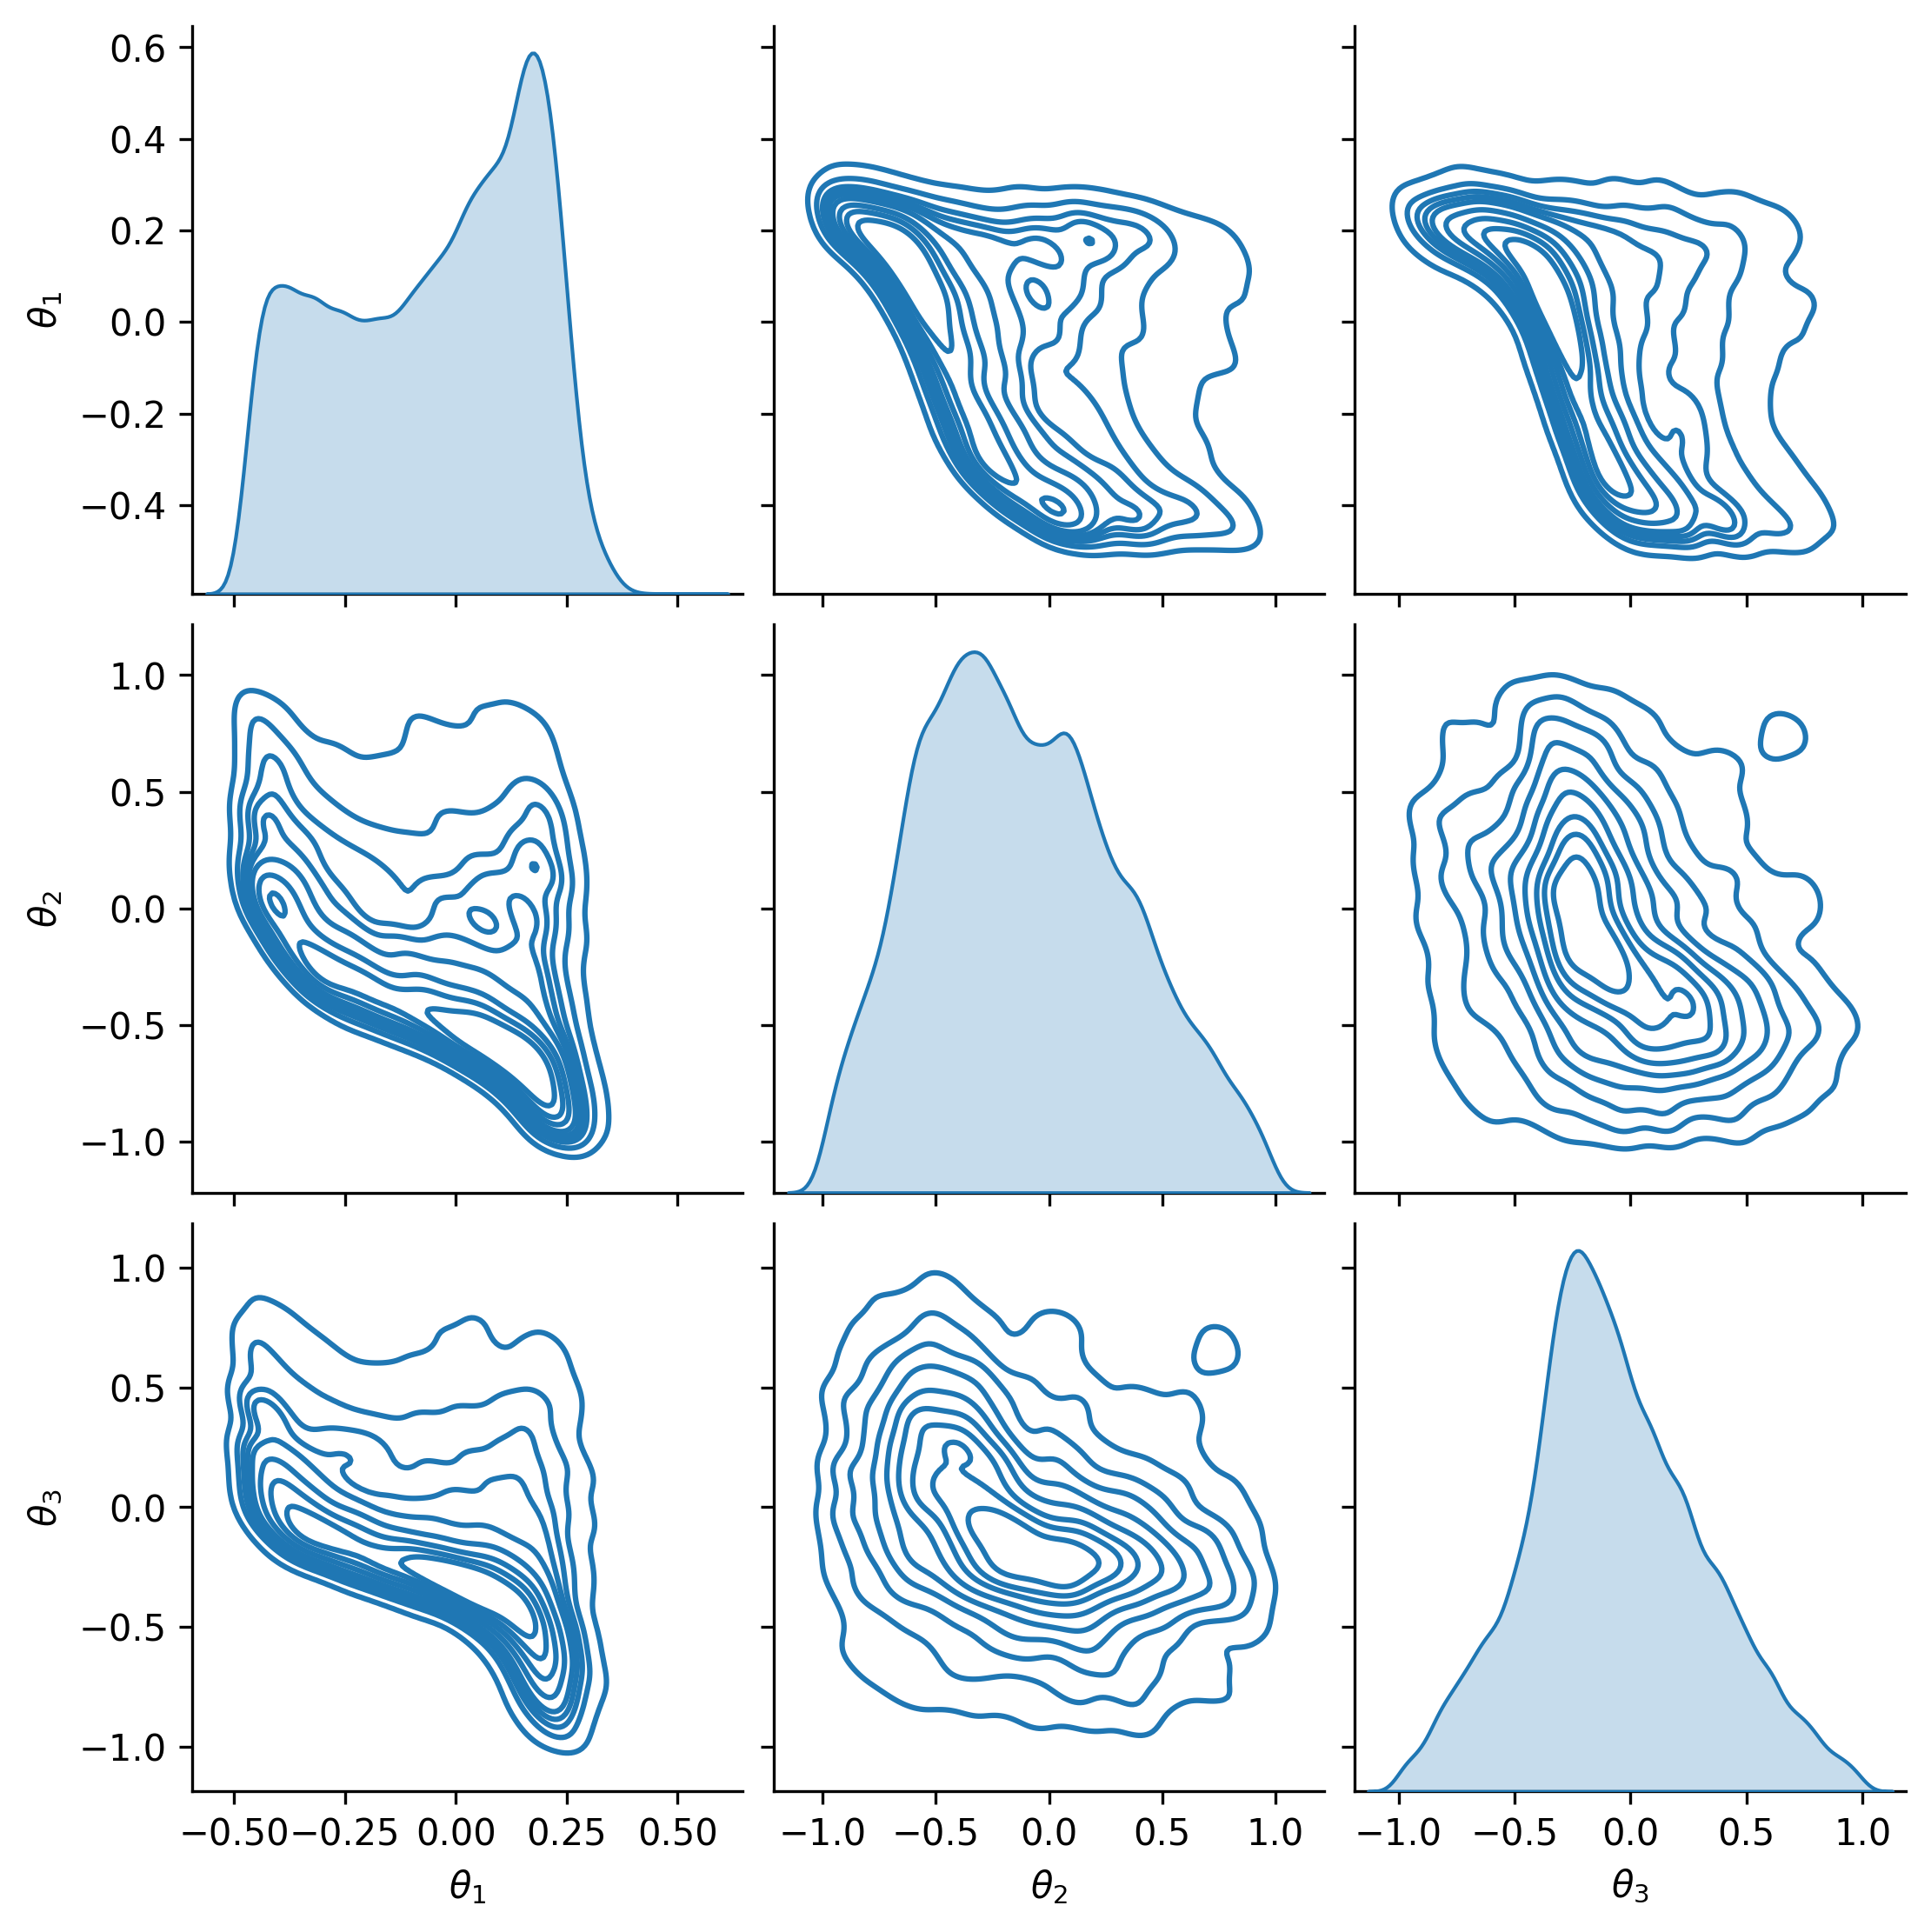
\includegraphics[width=1.0\linewidth]{Figures/appendix_figs/kde_model3_Stretch.png}
\caption{Pairs plots (with a kernel density style) for all calibrated parameters of Model 3. The presented data is from 5 ensembles (last 1000 steps of each chain), run with AI, an uninformative prior and 1 observation for evaluating the likelihood. The parameters as presented here are transformed for MCMC.}\label{fig_kde_model3_AI}
\end{figure}

%   MODEL 4

\begin{figure}[ht]
\centering
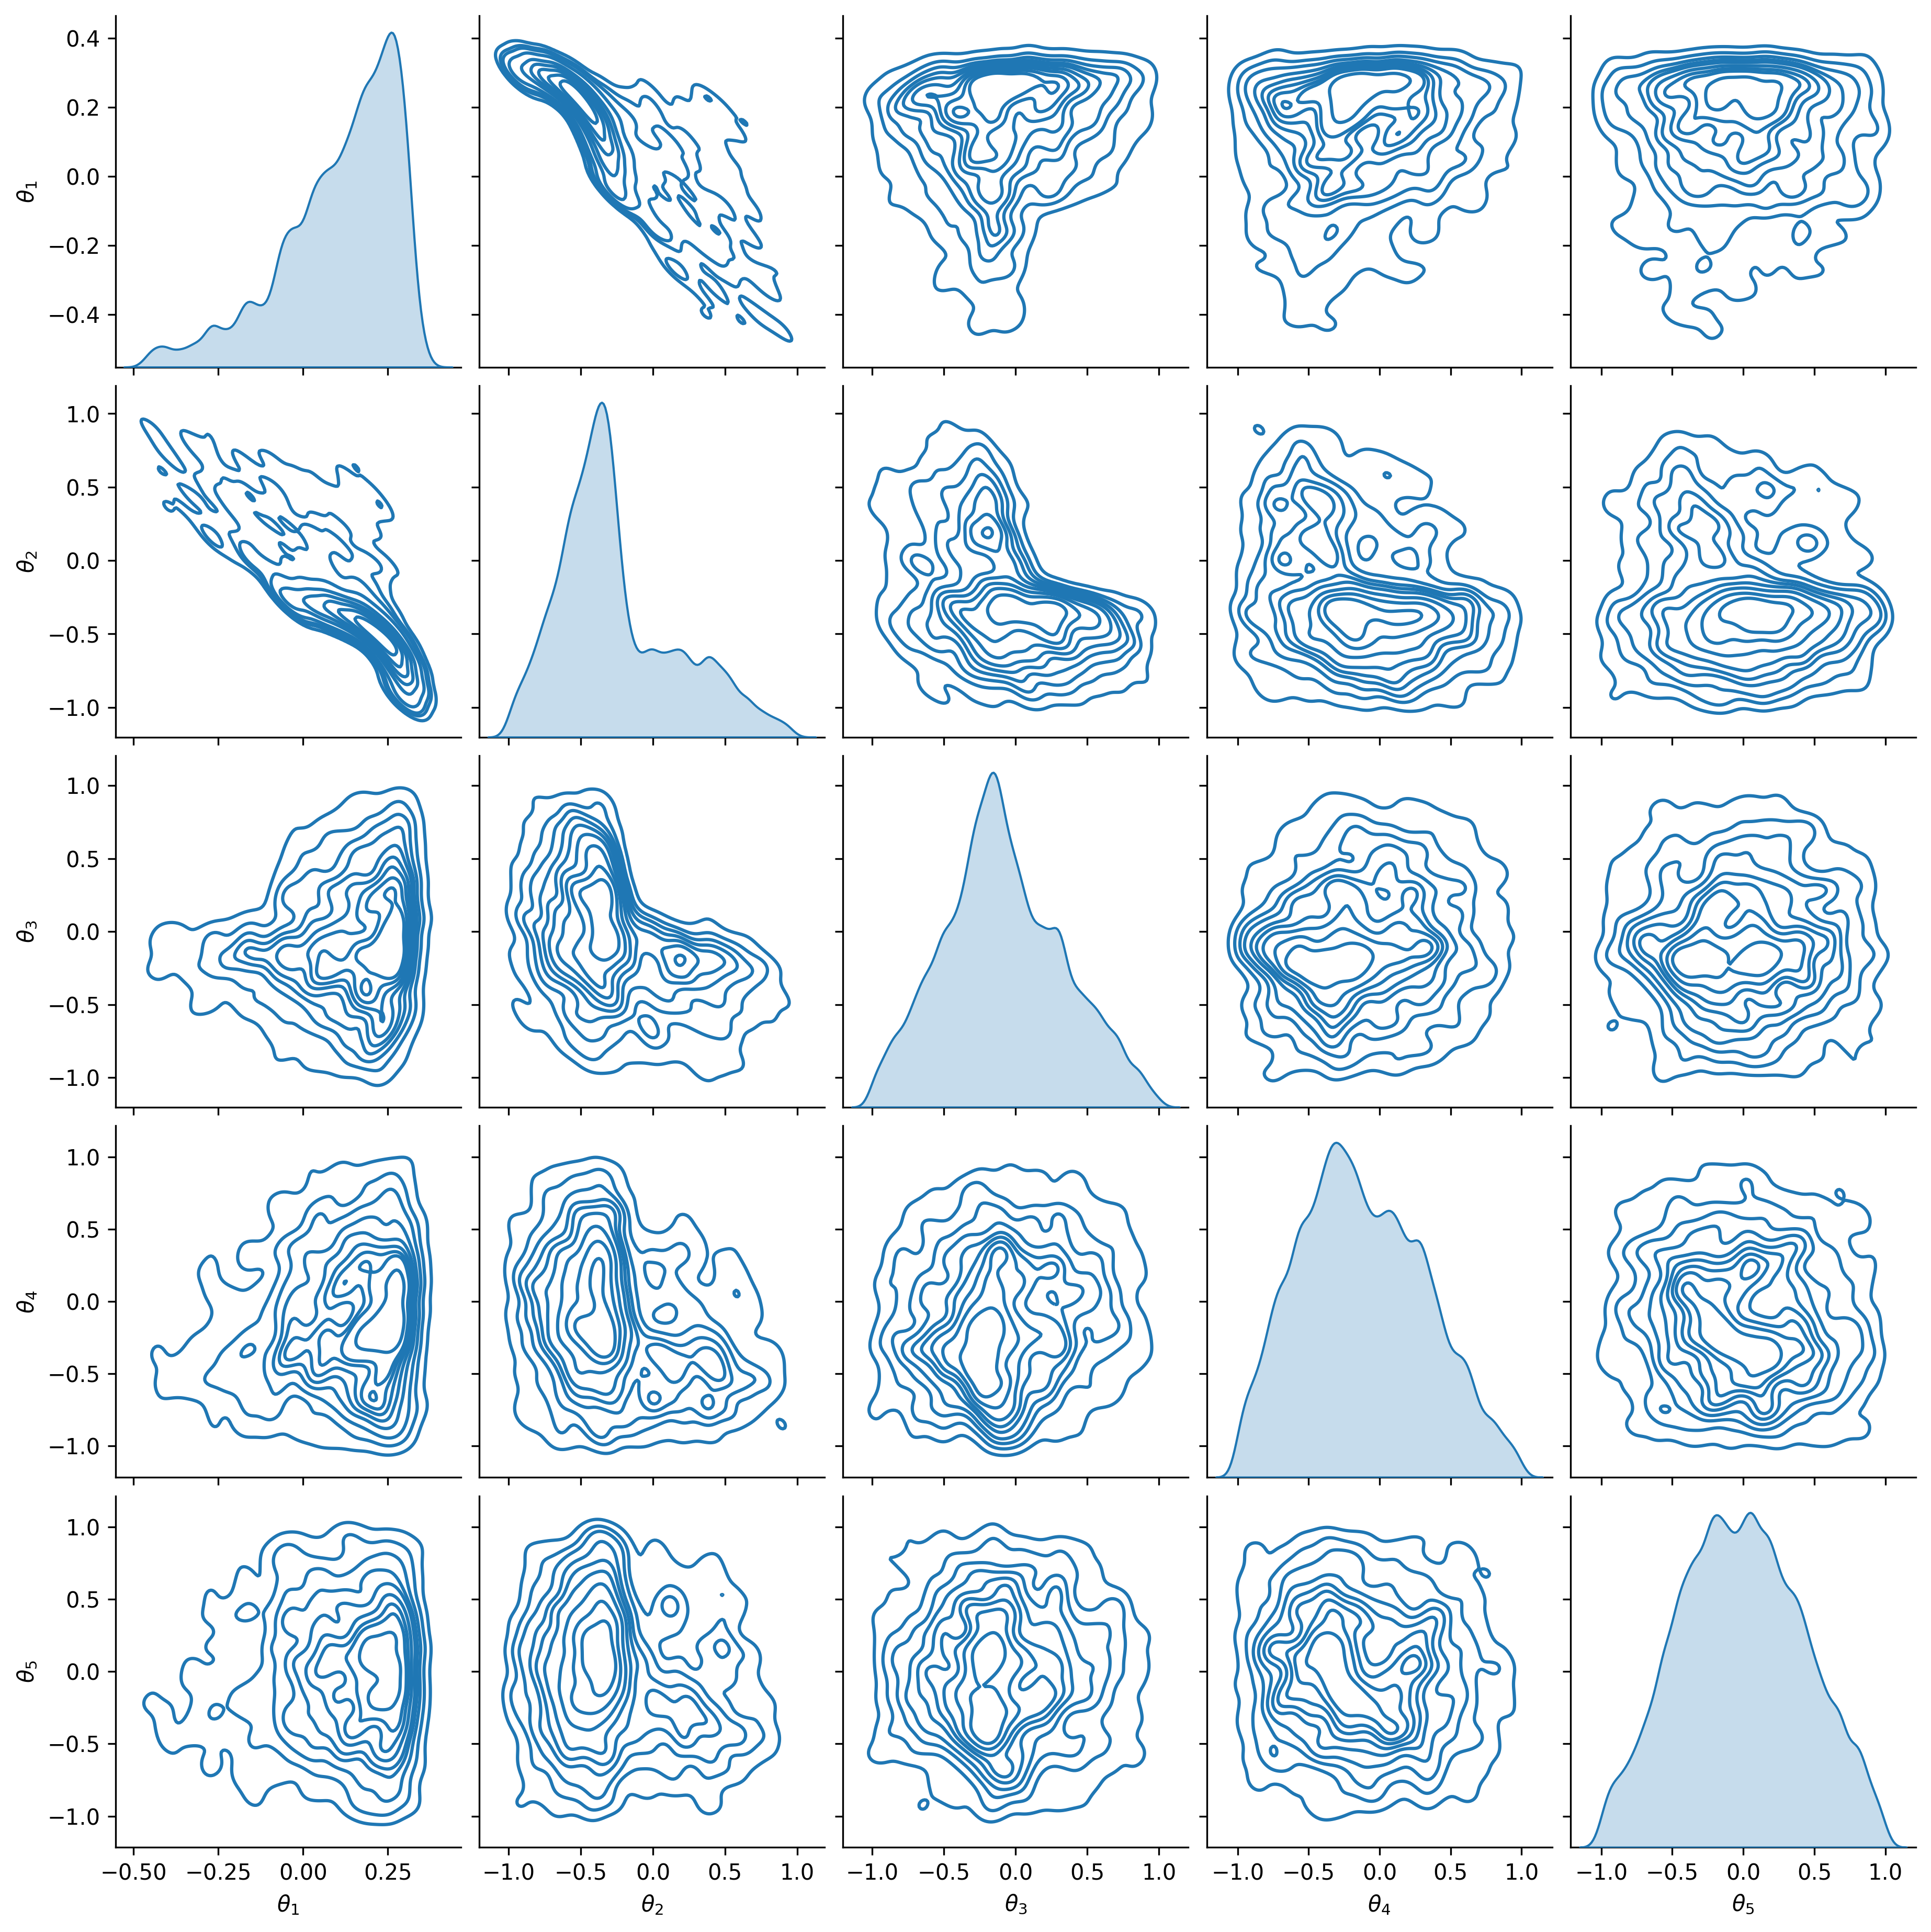
\includegraphics[width=1.0\linewidth]{Figures/appendix_figs/kde_model4_DE.png}
\caption{Pairs plots (with a kernel density style) for all calibrated parameters of Model 4. The presented data is from 5 ensembles (last 1000 steps of each chain), run with DE, an uninformative prior and 1 observation for evaluating the likelihood. The parameters as presented here are transformed for MCMC.}\label{fig_kde_model4_DE}
\end{figure}

\begin{figure}[ht]
\centering
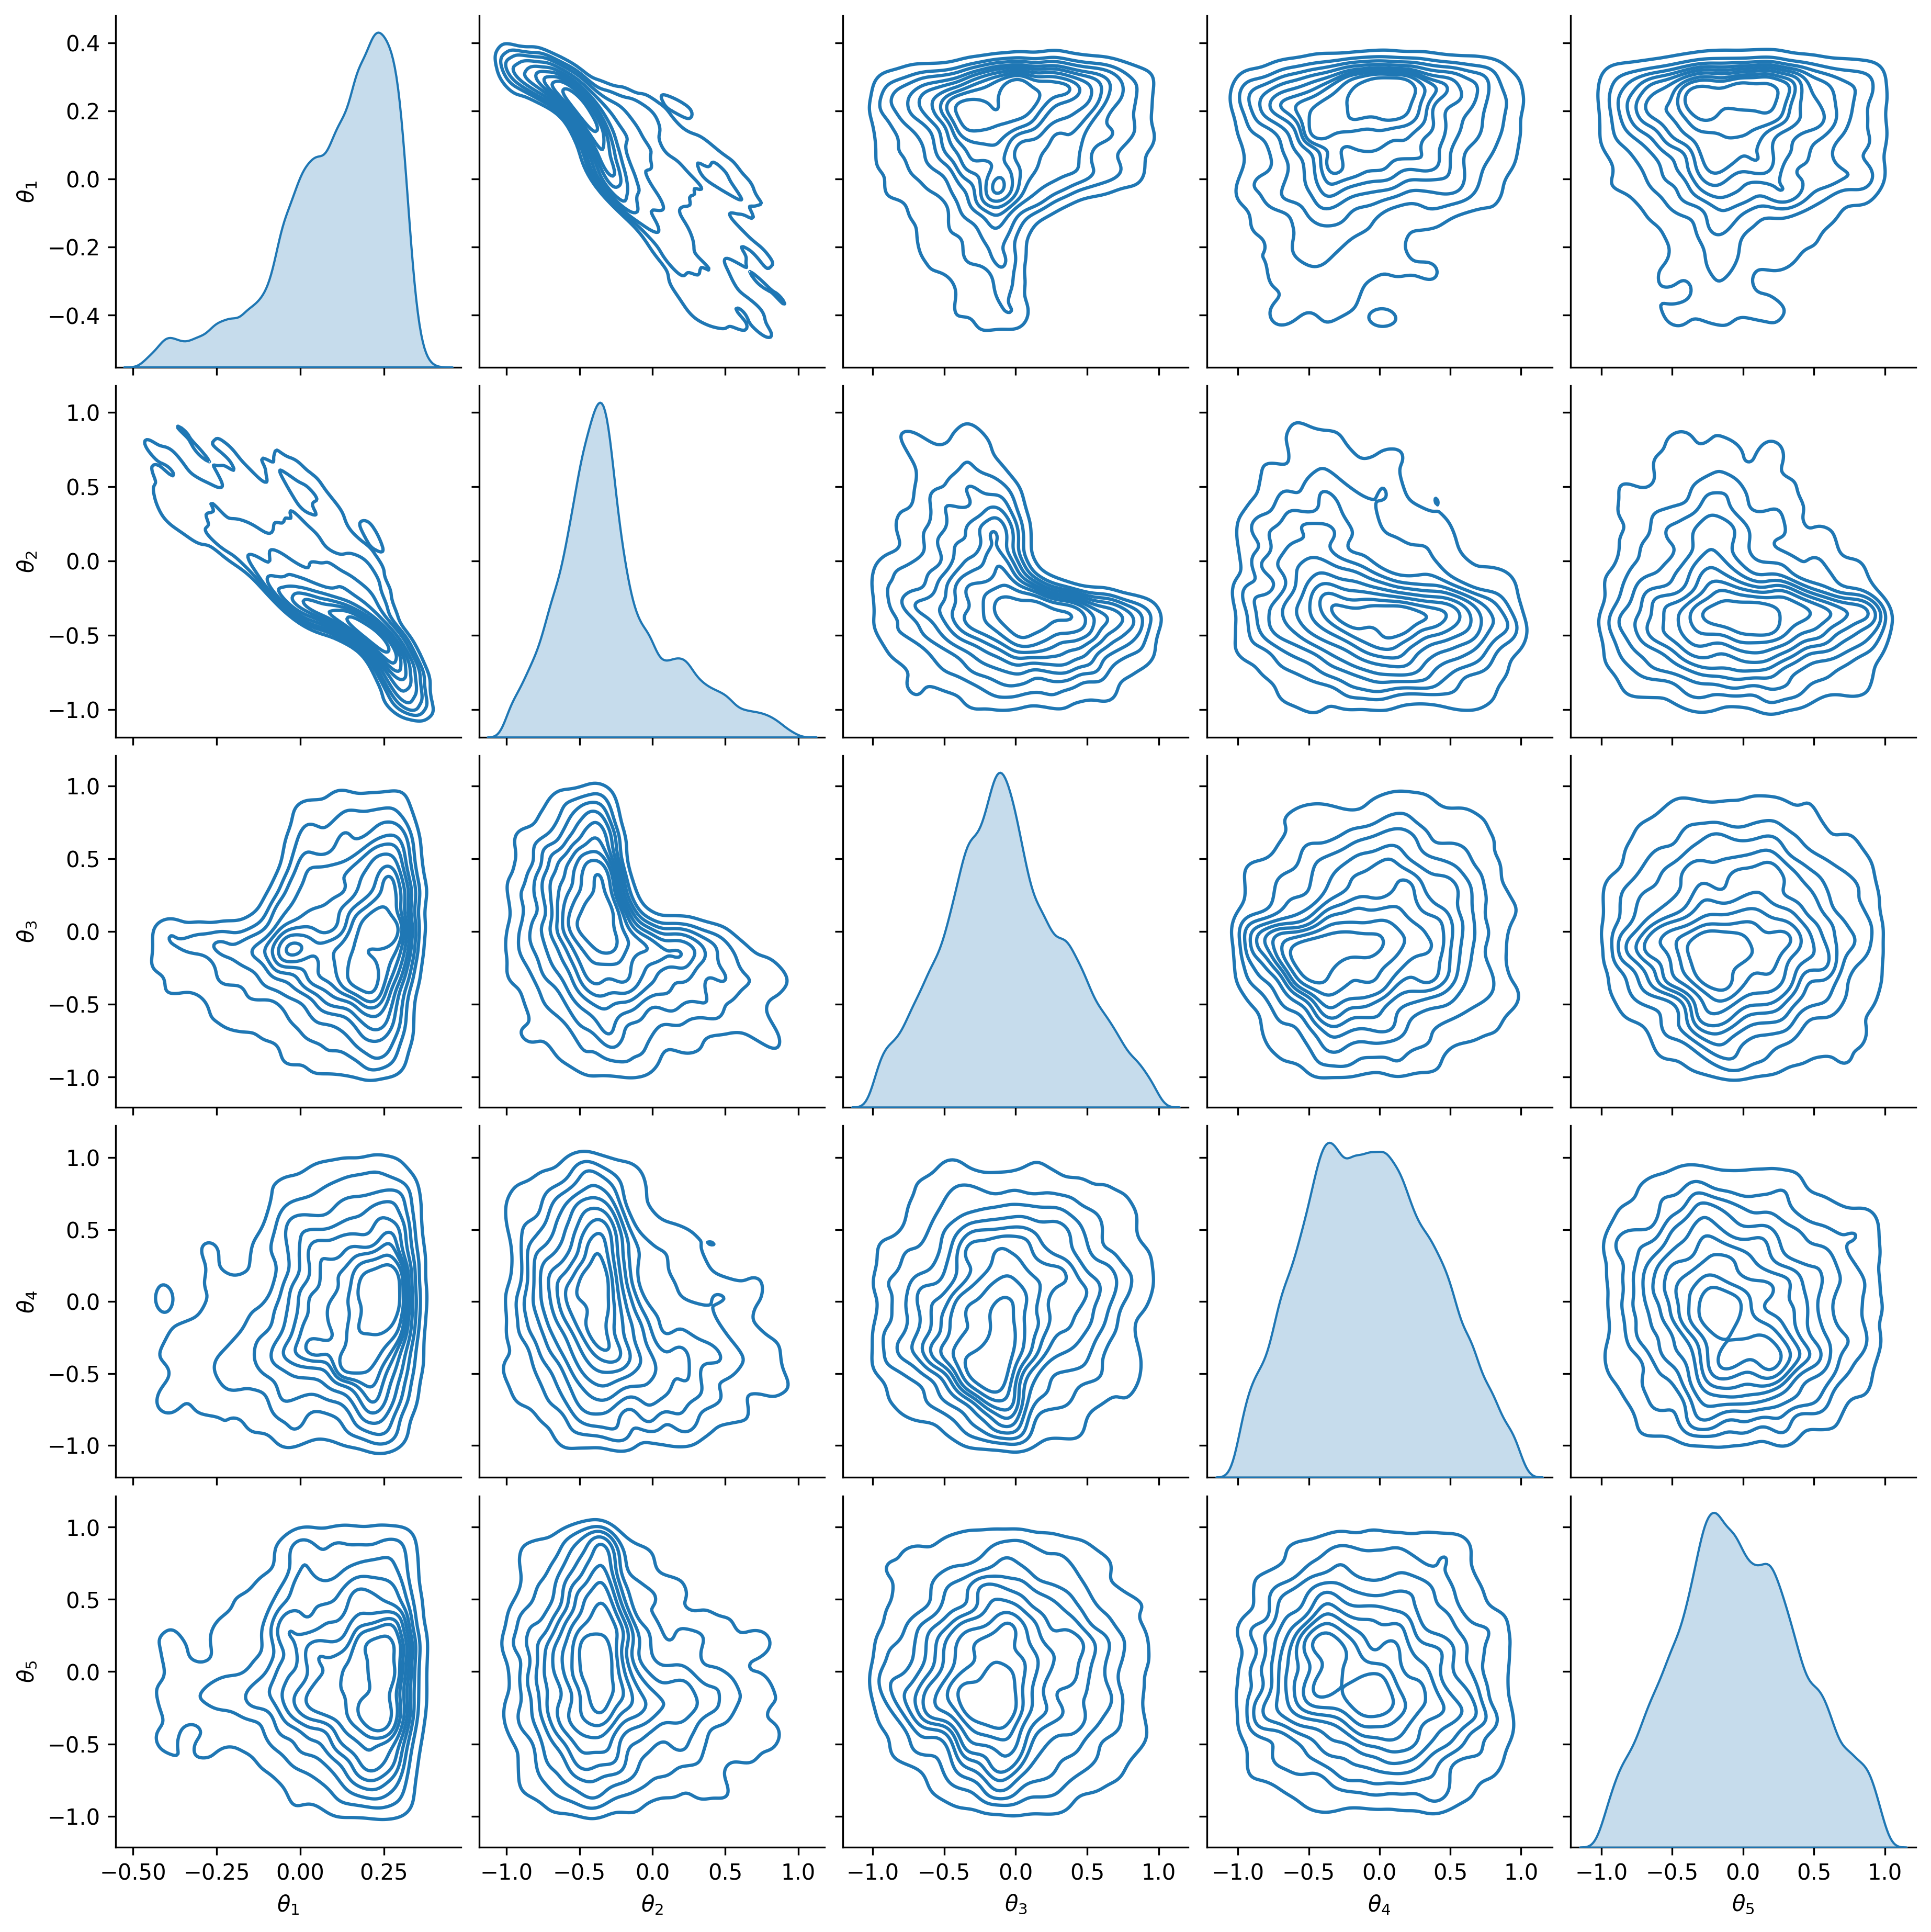
\includegraphics[width=1.0\linewidth]{Figures/appendix_figs/kde_model4_Stretch.png}
\caption{Pairs plots (with a kernel density style) for all calibrated parameters of Model 4. The presented data is from 5 ensembles (last 1000 steps of each chain), run with AI, an uninformative prior and 1 observation for evaluating the likelihood. The parameters as presented here are transformed for MCMC.}\label{fig_kde_model4_AI}
\end{figure}